%!TEX root=../document.tex

\section{Ergebnisse}
\label{sec:Ergebnisse}
Zur Umsetzung dieser Übung wurde das Tutorial von Android Guru befolgt. Der Sourcecode wurde importiert, wobei noch einige Fehler behoben werden mussten. Die App kann nun mit der REST Schnittstelle aus DezSys09 kommunizieren. \cite{GitHub-Repo09}

\subsection{Anbindung einer mobilen Applikation an die Webservice-Schnittstelle}
\label{subsec:Anbindung einer mobilen Applikation an die Webservice-Schnittstelle}
Das erste Problem trat beim Zugreifen auf localhost im Emulator auf. Nach einer kurzen Recherche im Internet konnte ein Post auf Stackoverflow weiterhelfen. \cite{AndroidLocalhost}
Im Simulator muss statt localhost die IP-Adresse 10.0.2.2 eingegeben werden.

Ein weiteres Problem war die Realisierung von DezSys09 mittels POST und JSON, während das Tutorial auf GET ausgelegt ist. In den Klassen LoginActivity und RegisterActivity muss noch das RequestParams Objekt auf ein JSONObject geändert werden.

\begin{lstlisting}[frame=single, language=java, caption=Ändern des RequestParams Objekts auf ein JSONObject]
ALT:
// Instantiate Http Request Param Object
RequestParams params = new RequestParams();

NEU:
JSONObject params = new JSONObject();
\end{lstlisting}

Nun muss das JSON-File noch mit angegebenen Daten befüllt werden.
\begin{lstlisting}[frame=single, language=java, caption=Ändern des RequestParams Objekts auf ein JSONObject]
StringEntity request = null;
try {
	request = new StringEntity(params.toString());
	request.setContentType(new BasicHeader(HTTP.CONTENT_TYPE, "application/json"));
} catch (UnsupportedEncodingException e) {
	e.printStackTrace();
}
\end{lstlisting}

Die Requestart wurde von GET und RequestParams auf POST und JSONObject geändert, die Variante der Verbindung muss noch von AsyncHttpClient geändert werden.

\begin{lstlisting}[frame=single, language=java, caption=Ändern des AsyncHttpClients]
ALT:
AsyncHttpClient client = new AsyncHttpClient();
client.get("http://192.168.2.2:9999/useraccount/login/dologin",params ,new AsyncHttpResponseHandler()

NEU:
AsyncHttpClient client = new AsyncHttpClient(); client.post(this.getApplicationContext(), "http://10.0.2.2:8080/register", request, "application/json", new TextHttpResponseHandler() {
\end{lstlisting}

Nun muss die onSuccess-Methode geändert werden.
\begin{lstlisting}[frame=single, language=java, caption=onSuccess Methode]
@Override
public void onSuccess(String response) {
// Hide Progress Dialog
prgDialog.hide();
try {
// JSON Object
JSONObject obj = new JSONObject(response);
// When the JSON response has status boolean value assigned with true
if(obj.getBoolean("status")){
Toast.makeText(getApplicationContext(), "You are successfully logged in!", Toast.LENGTH_LONG).show();
// Navigate to Home screen
navigatetoHomeActivity();
}
// Else display error message
else{
errorMsg.setText(obj.getString("error_msg"));
Toast.makeText(getApplicationContext(), obj.getString("error_msg"), Toast.LENGTH_LONG).show();
}
} catch (JSONException e) {
// TODO Auto-generated catch block
Toast.makeText(getApplicationContext(), "Error Occured [Server's JSON response might be invalid]!", Toast.LENGTH_LONG).show();
e.printStackTrace();
}
}
\end{lstlisting}

Die Registrierung wurde entsprechend angepasst.
\begin{lstlisting}[frame=single, language=java, caption=Neue Registrierung]
@Override
public void onSuccess(int statusCode, Header[] headers, String responseBody) {
	prgDialog.hide();
	// When Http response code is '201'
	if (statusCode == 201) {
		Toast.makeText(getApplicationContext(), responseBody, Toast.LENGTH_LONG).show();
		// Navigate to Home screen 		navigatetoLoginActivity(findViewById(android.R.id.content)); 	}
}
\end{lstlisting}

Der Login wurde entsprechend angepasst.
\begin{lstlisting}[frame=single, language=java, caption=Neue Registrierung]
@Override
public void onSuccess(int statusCode, Header[] headers, String responseBody) {
	prgDialog.hide();
	// When Http response code is '200'
	if(statusCode == 200) {
		Toast.makeText(getApplicationContext(), responseBody, Toast.LENGTH_LONG).show();
		// Navigate to Home screen
		navigatetoHomeActivity();
	}
}
\end{lstlisting}

%\subsection{Registierung von Benutzern}
%\label{subsec:Registierung von Benutzern}
%
%\subsection{Login und Anzeige einer Willkommensnachricht}
%\label{subsec:Login und Anzeige einer Willkommensnachricht}
%
%\subsection{Simulation bzw. Deployment auf mobilem Gerät}
%\label{subsec:Simulation bzw. Deployment auf mobilem Gerät}

\subsection{Ausführen der App mittels Simulationsumgebung}
\label{subsec:Ausführen der App mittels Simulationsumgebung}
Android Studio bringt neben den bereits genannten noch weitere nützliche integrierte Funktionen mit sich. Dazu gehört unter anderem die Simulation mittels Android Virtual Devices.
Um die Applikation auszuführen muss lediglich der „Play-Button“ betätigt werden, sofern keine Run-Konfiguration ausgewählt ist. Sollte sich kein Fenster für den Emulator öffnen, muss die Run-Konfiguration „Android Application“ ausgewählt werden. Nach einem erfolgreichen Starten der Run-Konfiguration sollte die folgende Maske zu sehen sein.

\begin{figure}[H]
	\begin{center}
		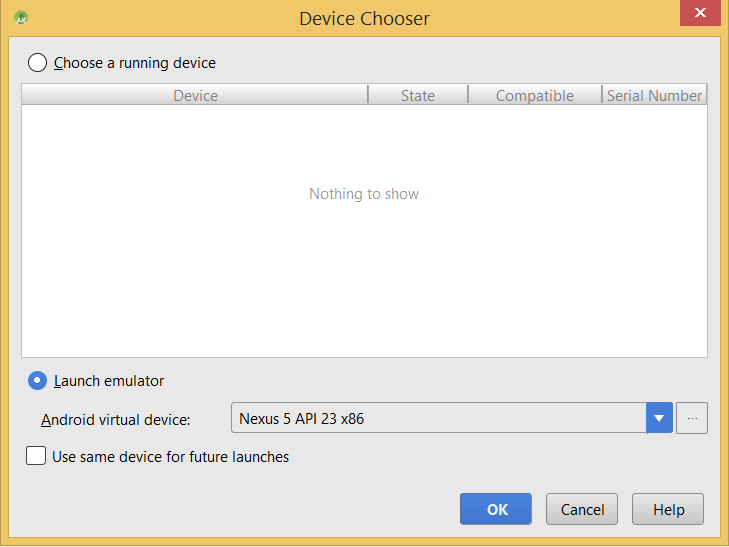
\includegraphics[width=1.0\linewidth]{images/device_chooser.png}
		\caption{Device Chooser}
		\label{device_chooser}
	\end{center}
\end{figure}

Sollte beim Punkt „Android virtual device“ noch kein Gerät ausgewählt sein, muss dieses erst über den Button mit den drei Punkten („…“) hinzugefügt werden. Dort angelangt sollte man den Button „Create Virtual Device…“ auffinden. Dieser wiederum öffnet die folgende Maske.

\begin{figure}[H]
	\begin{center}
		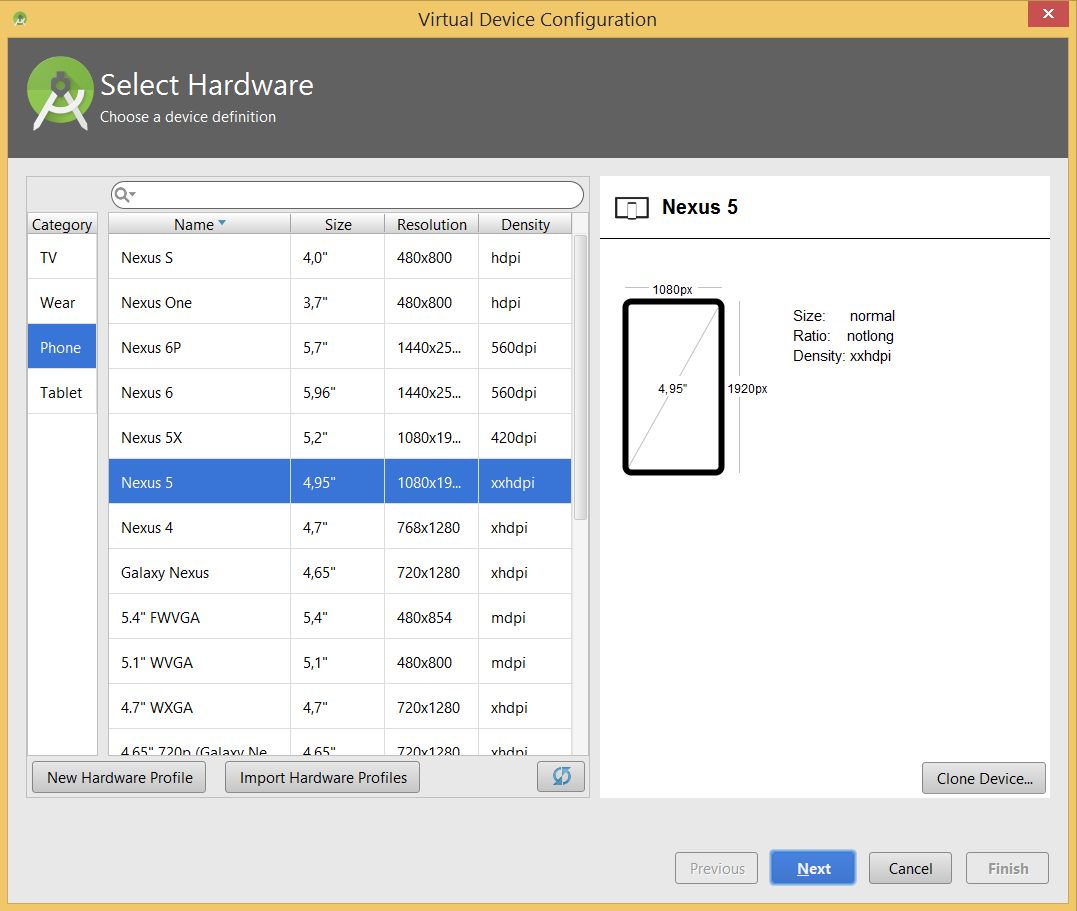
\includegraphics[width=1.0\linewidth]{images/new_device.png}
		\caption{Neues Device erstellen}
		\label{Neues Device erstellen}
	\end{center}
\end{figure}

Nun kann das entsprechende Gerät aus der Liste ausgewählt werden. Durch einen Klick auf „Next“ kann das zu installierende Image ausgewählt werden und durch einen erneuten Klick auf „Next“ gelangt man zur Settings-Seite. Nun sollte dort eine wichtige Einstellung überprüft werden. Diese ist in den erweiterten Einstellungen zu finden, welche über den Button „Show Advanced Settings“ angezeigt werden können. Konkret handelt es sich um die Checkbox „Enable Keyboard Input“, welche angehakt sein sollte. Dadurch ist es möglich jegliche Eingabe auf der Tastatur an das virtuelle Device weiterzuleiten.

\begin{figure}[H]
	\begin{center}
		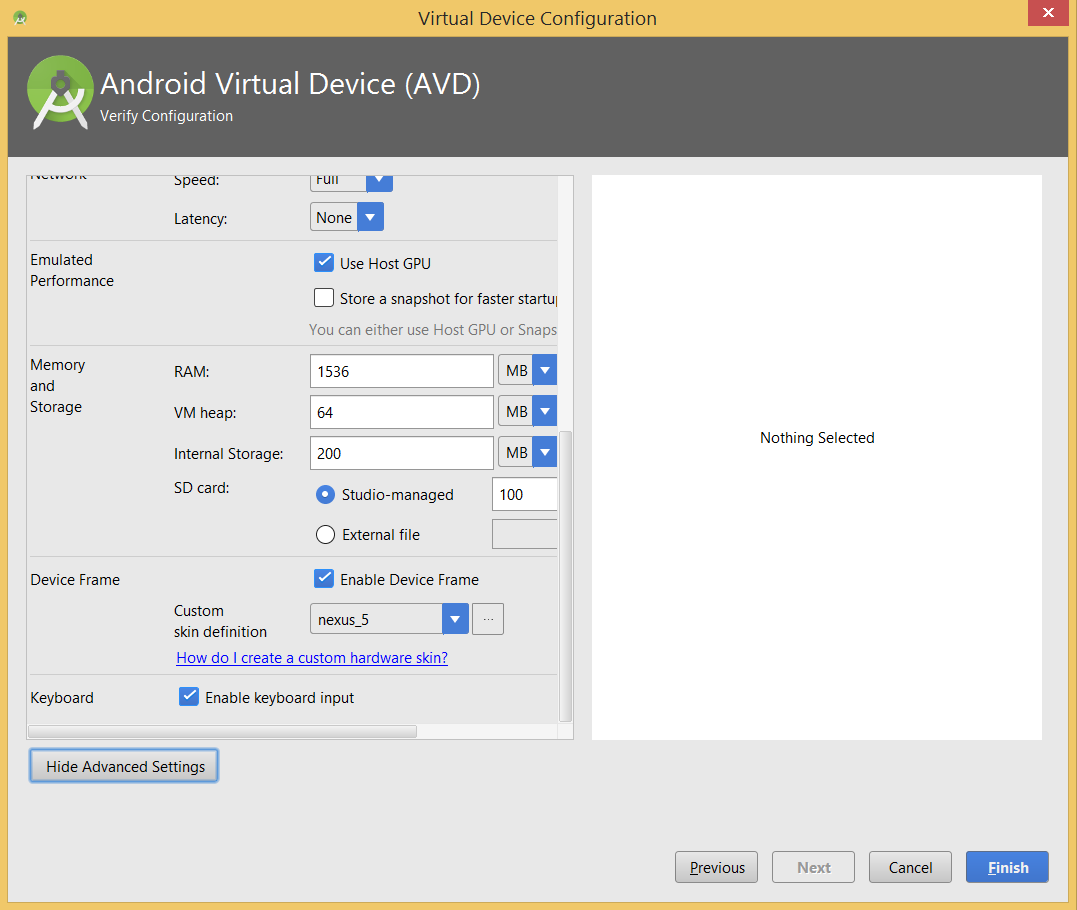
\includegraphics[width=1.0\linewidth]{images/key_input.png}
		\caption{Keyboard Input aktivieren}
		\label{Keyboard Input aktivieren}
	\end{center}
\end{figure}

Nun kann die Konfiguration über den Button „Finish“ abgeschlossen werden. Es sollte noch erwähnt werden, das Intel HAXM für das Ausführen des AVDs installiert sein muss. Dies wird allerdings meist bereits mit der Installation von Android Studio mitinstalliert.
Wird die „Android Application“ Run-Konfiguration nun erneut ausgeführt, sollte das erstellte Device in der Liste angeführt sein. Nun startet das AVD und nach einem erfolgreichen Boot-Vorgang wird die Applikation automatisch deployed und gestartet.

\subsection{Builden der Anwendung}
\label{subsec:Builden der Anwendung}
Das Builden der Applikation ist sehr einfach, da das von Android Studio erstellte Projekt ohnehin bereits Gradle verwendet. Um eine APK-Datei zu erzeugen kann eine neue „Gradle“ Run-Konfiguration mit Android Studio mit den folgenden Einstellungen erzeugt werden.

\begin{figure}[H]
	\begin{center}
		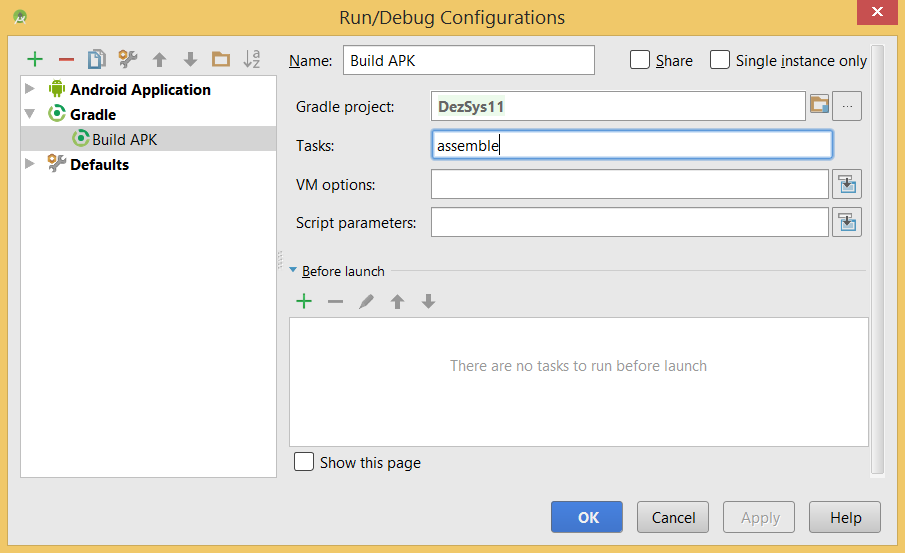
\includegraphics[width=1.0\linewidth]{images/run.png}
		\caption{Run-Konfigurationen}
		\label{Run-Konfigurationen}
	\end{center}
\end{figure}

Der Eintrag „Gradle project“ verweist dabei auf die Projektwurzel. (Project-Root)
Die Erstellte Run-Konfiguration kann nun ausgeführt werden und erstellt das APK-File in den Ordner app/build/outputs/apk.

\subsection{Link zum Repository}
\label{subsec:Link zum Repository}
Die Abgabe wurde, wie üblich, auf GitHub zur Verfügung gestellt. \cite{GitHub-Repo}


\newpage